\documentclass[10pt,letterpaper]{article}
\usepackage[top=0.85in,left=2.75in,footskip=0.75in,marginparwidth=2in]{geometry}

% use Unicode characters - try changing the option if you run into troubles with special characters (e.g. umlauts)
\usepackage[utf8]{inputenc}

% clean citations
\usepackage{cite}

% hyperref makes references clicky. use \url{www.example.com} or \href{www.example.com}{description} to add a clicky url
\usepackage{nameref,hyperref}

% line numbers
\usepackage[right]{lineno}

% improves typesetting in LaTeX
\usepackage{microtype}
\DisableLigatures[f]{encoding = *, family = * }

% text layout - change as needed
\raggedright
\setlength{\parindent}{0.5cm}
\textwidth 5.25in 
\textheight 8.75in

% Remove % for double line spacing
%\usepackage{setspace} 
%\doublespacing

% use adjustwidth environment to exceed text width (see examples in text)
\usepackage{changepage}

% adjust caption style
\usepackage[aboveskip=1pt,labelfont=bf,labelsep=period,singlelinecheck=off]{caption}

% remove brackets from references
\makeatletter
\renewcommand{\@biblabel}[1]{\quad#1.}
\makeatother

% headrule, footrule and page numbers
\usepackage{lastpage,fancyhdr,graphicx}
\usepackage{epstopdf}
\pagestyle{myheadings}
\pagestyle{fancy}
\fancyhf{}
\rfoot{\thepage/\pageref{LastPage}}
\renewcommand{\footrule}{\hrule height 2pt \vspace{2mm}}
\fancyheadoffset[L]{2.25in}
\fancyfootoffset[L]{2.25in}

% use \textcolor{color}{text} for colored text (e.g. highlight to-do areas)
\usepackage{color}

% define custom colors (this one is for figure captions)
\definecolor{Gray}{gray}{.25}

% this is required to include graphics
\usepackage{graphicx}

% use if you want to put caption to the side of the figure - see example in text
\usepackage{sidecap}

% use for have text wrap around figures
\usepackage{wrapfig}
\usepackage[pscoord]{eso-pic}
\usepackage[fulladjust]{marginnote}
\reversemarginpar

% for better-looking tables
\usepackage{booktabs}

% math utils
\usepackage{amsmath}

% symbols
\usepackage{gensymb}

% % citation aliases
% \usepackage{natbib}
% % https://tex.stackexchange.com/questions/323868/setting-two-different-aliases-name-2016-name-2016-with-defcitealias
% \newcommand{\mycitet}[1]{\citetalias{#1} (\citeyear{#1})}
% \newcommand{\mycitep}[1]{(\citetalias{#1} \citeyear{#1})}

% force floats in sections
\usepackage{float}

% document begins here
\begin{document}
\vspace*{0.35in}

% \defcitealias{arezh2018bodenbedeckung}{ARE}
% \defcitealias{asitvd2018structure}{ASIT VD}
% \defcitealias{bve2019mopube}{BVE}


% title goes here:
\begin{flushleft}
{\Large
\textbf\newline{}
}
\newline
% authors go here:
\\
% Mart\'i Bosch\textsuperscript{*},
% Maxence Locatelli,
% J\'er\^ome Chenal
% \\
% \bigskip
% Urban and Regional Planning Community (CEAT), \'Ecole Polytechnique F\'ed\'erale de Lausanne (EPFL), Lausanne, Switzerland
% \\ 
\bigskip
* Corresponding author: marti.bosch@epfl.ch

\end{flushleft}

\section*{Abstract}

% A reusable computational workflow to assess urban heat islands in Python

% We show how remote sensing data, air temperature measurements and cadastral datasets can be used to simulate urban heat islands with the urban cooling model of the InVEST software platform.

% The global increase of urban populations brings new challenges to urban planning and policy making.
% In the context of climate change, urban heat mitigation is a major priority for many cities that are exposed to rising temperatures and heat waves.
% To that end, it is central to understand the relationship between the spatial pattern of urban land cover and the intensity and distribution of urban heat islands.
% % With the increasing availability of satellite imagery,
% The former can be easily evaluated given the wide availability of cadastral and land use/land cover dataset. In order to estimate the latter, most studies exploit remote sensing data to compute the land surface temperature.
% While most research suggests a significant relationships between the spatial composition and configuration of urban tree canopy and the distribution of land surface temperature, many contradicting results regarding the magnitude and direction of such correlations have been reported.
% Overall, two major weaknesses might be noted in such approaches. 
% On the one hand, land surface temperature cannot fully represent human exposure to heat, which is better represented by air temperature.
% On the other hand, and most importantly, even when accounting for spatial autocorrelation, statistical approaches are hard to relate to the physical mechanisms driving urban heat islands and therefore can hardly elighten the understanding of the phenomenon.

% % The proposed approach represents two major improvements over existing approaches.
% % On the one hand, air temperature estimates based on station measurements provide more suitable representation of human exposure to heat.
% % On the one hand, air temperature provides a better representation of the human exposure to heat than land surface temperature.
% % On the other hand, even when accounting for spatial autocorrelation, statistical approaches are hard to relate to the physical mechanisms driving urban heat islands and therefore can hardly elighten the understanding of the phenomenon.
% The aim of this presentation is to propose a reusable computational workflow to model urban heat islands that addresses the shortcomings reviewed above.
% The approach is based on the urban cooling model of the InVEST software platform, which models the urban air temperature as a function of three main physical mechanisms, namely the shade, evapotranspiration and albedo.
% The proposed method requires four main inputs, which are a categorical land cover raster map, a biophysical table containing model information of each LULC class of the map, a high-resolution tree canopy map, and a reference evapotranspiration raster. The computational workflow consists of three steps.
% Firstly, a supervised learning approach combines openly available satellite data and air temperature measurements from monitoring stations in order to downscale the latter and obtain a map of air temperature at an appropriate resolution. Such map will then serve two purposes, i.e., to compute the input reference evapotranspiration raster, and to calibrate the urban cooling model.
% Secondly, in order to better represent for the spatial heterogeneity of urban landscapes, the land cover raster map is coupled with the tree canopy map to refine the land cover classes depending on their proportion of tree cover. For instance, pixels of a ``sidewalk'' class could be reclassified to further distinguish pixels of a ``sidewalk with high tree cover'' and ``sidewalk with low tree cover''. The reclassification will be accounted for in the biophysical table so that pixels with high tree cover have greater shading coefficients.
% Finally, the preprocessed data will be fed into the urban cooling model to achieve a distribution of air temperature that mimics the patterns observed empirically.

% An example application to the study of urban heat islands in the Swiss urban agglomeration of Lausanne will be presented in order to show how the computational workflow might be applied in realistic settings.
% Additionally, the proposed approach aims at providing a reusable method with moderate data requirements that can be applied to very distinct urban areas, and might thus provide new insights into many of the contradicting results encountered in the literature.



% now start line numbers
\linenumbers

% the * after section prevents numbering
\section*{Introduction}

% Distinction: three types of UHI: urban boundary layer, urban canopy layer \cite{oke1976distinction}

% ``We know that simply increasing the percent cover of greenspace leads to a reduction of temperatures; this relationship is very consistent. What is less known, however, is the effects of the spatial configuration of that greenspace on urban temperatures'' \cite[page 2]{zhou2017effects}
% The complexity of such relationship might only be understood by means of a spatially-explicit analysis. Several studies have addressed the effects of landscape composition and pattern on land surface temperature (LST), e.g., derived from satellite imagery, by means of statistical approaches (e.g., ordinary regressions or spatial autoregressions). 
% non-linear interplay between landscape patterns and ecological processes \cite{du2016quantifying}
% Note that while most studies that use single-level statistical models suggest that landscape composition has greater influence on LST than landscape configuration, the multi-level models used by Du et al. \cite{du2016quantifying} suggest the opposite. Why? (i) group-based configuration metrics consider the autocorrelations of the configuration metrics, and (ii) the aggregation effects of the groups and the individual effects of the pixels are distinguished by the multi-level models.
% Note however further limitations of statistical approaches in general:
% ``Our results from the comparison of the two cities indicated that the spatial configuration of trees may have different effects on LST in cities with different climatic conditions'' \cite[page 6]{zhou2017effects}
% This might be due to the fact that the relative contributions of the two main cooling mechanisms associated to urban trees, namely shading and evapotranspiration, can be related to the different climatic conditions of the modelled cities \cite{zhou2017effects}.
% Nevertheless, the statistical approaches employed in such studies (e.g., ordinary regressions or spatial autoregressions with LST as response and landscape metrics as explanatory variables) do not explicitly reflect the physical mechanisms beyond the urban heat island phenomena.


% Urban areas are heterogeneous in their distribution of built and natural components \cite{cadenasso2007spatial}, especially relevant to urban climate studies \cite{stewart2012local}.

% Distinction from the landscape ecology perspective: composition metrics (percent cover of green space) and configuration metrics (distribution of patches).

% Another advantage: cities with very similar climatic conditions, and very homogeneous data

% Also issue of how the extents are defined

% efficiency in cooling: decrease in degrees of LST with every 1% increase in tree cover (page 6 of \cite{zhou2017effects})

% NDVI vs tree cover: NDVI includes both trees and grass/lawns. Note that grass is less effective than tree canopy for LST cooling

% greening \cite{jabareen2006sustainable}


\section*{Materials and Methods}

\subsection*{Study area and land use/land cover data}



\subsection*{Simulation with the InVEST urban cooling model}

The second approach to simulate the spatial distribution of UHI employs the InVEST urban cooling model (version 3.8.0) \cite{sharp2020invest}, which is based on the heat mitigation provided by shade, evapotranspiration and albedo.
The main inputs are a LULC raster map, a reference evapotranspiration raster and a biophysical table containing model information of each LULC class of the map. Each row of the biophysical table represents a LULC class, and features the following columns:

\begin{itemize}
\item \texttt{lucode} the LULC class code as represented in the LULC raster map
\item \texttt{Shade} a value between 0 and 1 representing the proportion of tree cover in such LULC class
\item \texttt{Kc} the evapotranspiration coefficient
\item \texttt{Albedo} a value between 0 and 1 representing the proportion of solar radiation directly reflected by the LULC class
\item \texttt{Green\_area} whether the LULC class should be considered a green area
\item \texttt{Building\_intensity} a value between 0 and 1 representing the ratio between floor area and land area
\end{itemize}

In order to simulate the spatial distribution of $T_{air}$, the model requires two additional inputs. The first is the rural reference temperature $T_{ref}$, where the UHI effect is not observed, e.g., in the rural surroundings of the city. The second is the magnitude of the urban heat island effect $UHI_{max}$, namely the difference between the rural refrence temperature and the maximum $T_{air}$ observed in the city center.



\subsubsection*{Model description}

The data inputs described above are then used to compute the cooling capacity index, which is based on the physical mechanisms that contribute to cooling urban temperatures. More precisely, the cooling capacity index used in InVEST urban cooling model builds upon the indices proposed by Zardo et al. \cite{zardo2017estimating}, which are based on shading and evapotranspiration, and extends them by adding a factor to account for the albedo.
For each pixel $i$ of the LULC raster map, the cooling capacity index is computed as in:

\begin{equation}
  \label{eq:cooling-capacity}
  CC_i = w_{S} \cdot \textrm{S}_i + w_{AL} \cdot \textrm{AL}_i + w_{ET} \cdot \textrm{ETI}_i
\end{equation}

where $S_i$, $AL_i$ and $ETI_i$ respectively represent the tree shading, albedo and evapotranspiration values of pixel $i$ as defined in the biophysical table, and $w_{S}$, $w_{AL}$ and $w_{ET}$ represent the weights attributed to each component respectively.
The values of $S_i$ and $AL_i$ are retrieved from the biophysical table according to the LULC class of the pixel $i$ (see Appendix~\ref{table-biophysical}).
The tree shading coefficient corresponds to the average proportion of tree cover in all the 10~m pixels of each LULC class, which has been computed by coupling the 1~m binary tree canopy mask with the rasterized 10~m LULC map.
The albedo coefficients are based on the local climate zone classification by Steward and Oke \cite{stewart2012local}.

% \subsubsection*{Evapotranspiration}

The evapotranspiration index $ETI$ is computed as a normalized value of the potential evapotranspiration as in:

\begin{equation}
  \label{eq:evapotranspiration-index}
  ETI = \frac{K_c \cdot ET_{ref}}{ET_{max}}
\end{equation}

where $K_c$ is the evapotranspiration coefficient, $ET_{ref}$ is the reference evapotranspiration raster for the period and area of interest and $ET_{max}$ is the maximum evapotranspiration value observed in the area of interest.

% \paragraph{Adjustment of the crop coefficient}

In line with the studies of Nistor et al. \cite{nistor2015compute,nistor2016climate,nistor2016mapping}, the evapotranspiration coefficients are attributed to each LULC class by distinguishing four cases, namely the crop coefficient for single crops for vegetation LULC classes, the water evaporation coefficient for surface water, the rock and soil evaporation coefficient for bare soils and rocks, and evaporation coefficients for artificial LULC classes (e.g., urban areas).
The evapotranspiration coefficients attributed to the LULC classes of the Swiss cadastral survey are listed in Appendix~\ref{table-biophysical}.

% \paragraph{Computation of the evapotranspiration}

Following the recommendations of Allen et al. \cite{allen1998crop}, the daily evapotranspiration $ET_{ref}$ (in $mm/day$) has been estimated for each pixel using the Hargreaves equation \cite{hargreaves1985reference} as in:

\begin{equation}
  \label{eq:ref-evapotranspiration}
  ET_{ref} = 0.0023 \cdot (T_{avg} + 17.8) \cdot (T_{max} - T_{min})^{0.5} \cdot R_a
\end{equation}

where $T_{avg}$, $T_{max}$ and $T_{min}$ respectively correspond to the average, maximum and minimum $T_{air}$ (in \degree C) of each day and $R_a$ is the extraterrestrial radiation (in $mm/day$), which is in turn estimated for the latitude of Lausanne (i.e., 46.519833\degree) for each date following the methods of Allen et al. \cite[Equation 21]{allen1998crop}.
The temperature values of each day have been extracted from the inventory of gridded datasets provided by the Federal Office of Meteorology and Climatology (MeteoSwiss), which feature the minimum, average and maximum daily $T_{air}$ for the extent of the whole country at a resolution of 1~km. Such a dataset is obtained by interpolating 100 $T_{air}$ stations accross Switzerland (including the MeteoSwiss Pully station) based on non-linear thermal profiles of major basins and non-Euclidean distance weighting that accounts for terrain effects \cite{frei2014interpolation}.

In order to account for the cooling effect of large green spaces, the computed cooling capacity index of pixels that are part of large green areas ($>$ 2~ha) is adjusted as in:

\begin{equation}
  \label{eq:cooling-capacity-green}
  CC_i^{green} = \sum_{j \in \Omega_i} g_i \cdot CC_j \cdot e^{-\frac{d(i, j)}{d_{cool}}}
\end{equation}

where $g_i$ is 1 when the pixel $i$ is a green area and 0 otherwise (as defined in the biophyisical table), $d(i, j)$ is the distance between pixels $i$ and $j$, $d_{cool}$ is a parameter that defines the distance over which a green space has a cooling effect, and $\Omega_i$ is the set of pixels whose distance to $i$ is lower than $d_{cool}$.

Then, a heat mitigation index is computed as:

\begin{equation}
  \label{eq:heat-mitigation index}
  HM_i = \begin{cases}
    CC_i & \; if \;\; i \; \textrm{is part of a large green area} \;\; or \;\; CC_i > CC_i^{green} \\[.5em]
    CC_i^{green} & \; otherwise \\
    \end{cases}
\end{equation}

which is employed to compute the $T_i$ for each pixel $i$ of the study area as in:

\begin{equation}
  \label{eq:tair-nomix}
  T_i^{no \, mix} = T_{ref} + (1 - HM_i) \cdot UHI_{max}
\end{equation}

where $T_{ref}$ and $UHI_{max}$ are the rural reference temperature and the magnitude of the UHI effect respectively, as described above.
Finally, the $T_{air}$ values of each pixel $T_i^{no \, mix}$ are spatially averaged using a Gaussian function with a kernel radius $r$ defined by the user.


\subsubsection*{Calibration and evaluation of the model}




\subsection*{Refining LULC classes based on tree cover and building density}
\label{sec:refin-lulc-class}

To better account for the spatial heterogeneity of cities, a procedure to redefine the LULC classes from the cadastral survey has been designed, which further distinguishes the LULC classes depending on their proportional cover of both trees and buildings. Such reclassification is based on combining the 10~m raster LULC map with two 1~m binary raster masks, one for the tree canopy raster and another for the buildings. % , and consists of three main steps.
The 1~m binary tree canopy mask has been derived from the SWISSIMAGE orthomosaic \cite{swisstopo2019swissimage}, by means of the Python library DetecTree \cite{bosch2020detectree}, which implements the methods proposed by Yang et al. \cite{yang2009tree}. On the other hand, the 1~m binary building mask has been obtained by rasterizing the buildings of the vector cadastral survey \cite{asitvd2018structure}.

% The reclassification procedure consists of three steps.
% % First, for each LULC class, the set of 10m pixels of such class is coupled with the tree canopy and building masks
% Firstly, each 10~m pixel is coupled with the tree canopy and building masks in order to respectively compute its proportion of tree and building cover.
% % Secondly, each LULC class is further refined into a set of subclasses depending on the joint distribution of tree cover and building cover of its 10~m pixels, e.g., the ``sidewalk'' LULC code might be further refined into ``sidewalk with low tree/low building cover'', ``sidewalk with low tree/high building cover'', ``sidewalk with high tree/low building cover'' and ``sidewalk with high tree/high building cover''. %  its set of 10~m pixels are % the 10m pixels of each LULC class are grouped into equally-spaced bins according to their proportion of tree cover
% Secondly, the set of 10~m pixels of each LULC class are grouped into a set of bins to form two histograms, one based on their proportion of tree cover and the other analogously for the building cover.
% % which groups the 10~m pixels of each LULC class into an increasing number of equally-spaced bins according to their proportion of tree cover, until adding an extra bin results in having a bin whose number of samples is lower than certain threshold.
% The number of bins is determined by means of an iterative procedure which distributes the 10~m pixels into an increasing number of equally-spaced bins until adding an extra bin results in having a bin whose number of samples is lower than certain threshold.
% After empirical exploration, a threshold value of 3~\% has been manually chosen with the aim of obtaining a set of refined LULC codes that can be interpreted easily.
% % cartesian product
% Finally, the two histograms are joined so that each LULC class is further refined into a set of subclasses, e.g., the ``sidewalk'' LULC code might be further refined into ``sidewalk with low tree/low building cover'', ``sidewalk with low tree/high building cover'', ``sidewalk with high tree/low building cover'' and ``sidewalk with high tree/high building cover''.
The reclassification procedure consists of three steps.
Firstly, each 10~m pixel is coupled with the tree canopy and building masks in order to respectively compute its proportion of tree and building cover.
Secondly, the set of 10~m pixels of each LULC class are grouped into a user-defined set of bins to form two histograms, one based on their proportion of tree cover and the other analogously for the building cover.
% cartesian product
Finally, the two histograms are joined so that each LULC class is further refined into a set of subclasses. For example, if two bins were used for both the tree and building cover, the ``sidewalk'' LULC code might be further refined into ``sidewalk with low tree/low building cover'', ``sidewalk with low tree/high building cover'', ``sidewalk with high tree/low building cover'' and ``sidewalk with high tree/high building cover''.
In the present work, four equally spaced bins have been used to reclassify both the tree and building cover in order to obtain a more fine-grained LULC representation.

\subsection*{Generation of greening scenarios}

% One of the main advantages of using models based on biophysical mechanisms is that they allow for reasonable
Departing from the refined LULC map, a set of synthetic scenarios will be simulated by altering the LULC classes of certain pixels in a way that corresponds to reasonable transformations that could occcur in urban areas.
More precisely, in order to mimic scenarios of urban greening, pixels whose base LULC class corresponds to roads, sidewalks, traffic islands and other impervious surfaces will be changed to the LULC code that has the same base class but with the highest tree cover, e.g.,  pixels of a post-refinement class ``sidewalk with low tree/low building cover'' would be changed to ``sidewalk with high tree/low building cover''.
% TODO: limit such that the proportion of tree canopy cover and the proportion of building cover (i.e., "shade" + "bulding_intensity") does not amount to more than 100~\%
% TODO: randomized

% with two main objectives. The first objective is to use the scenarios to explore the relationships between spatial patterns in both composition and configuration of trees and the distribution of air temperature simulated with the urban cooling model. The second objective is to inform policy-making.
% In order to explore the relationships between spatial pattern of the tree canopy in each scenario and its respective distribution of air temperature simulated with the urban cooling model.
In order to quantify spatial pattern of the tree canopy of each scenario, a set of spatial metrics from landscape ecology \cite{o1988indices,mcgarigal2012fragstats} will be computed for the pixels whose post-refinement LULC class has a high tree canopy cover.  % over a certain threshold.
% deux pixels adjacents forment une canopée continue. Pour arriver à une telle conclusion, une typologie d’arbre est fixée. Sur recommandations de la Direction des ressources et du patrimoine naturel du canton de Vaud (DGE), une canopée coninue serait constituer d’arbres disposant d’une couronne sphérique de 5m de rayon, espacés chacun de 10m. Au vue de la dimension des pixels issus de la couche reclassifée (100 m 2 ), une telle typologie d’arbre correspondrait à une canopée de 75 m 2 , soit un degré de recouvrement de 75%
Following the advice given by the directorate of resoures and natural heritage in the Canton of Vaud (DGE-DIRNA), the threshold over which a pixel is considered to have a high tree canopy cover has been set to 75~\%, which corresponds to placing trees of a spheric crown with a 5~m radius spaced 10~m from one another so that they form a continuous canopy.
Based on related studies, four spatial metrics have been chosen to quantify both the composition and oconfiguration of the tree canopy, which are listed in \autoref{tab:selected-metrics}. The proportion of landscape (PLAND) of pixels with high tree canopy cover serves to quantify the composition aspects, while the configuration is quantified by means of the mean patch size (MPS), edge density (ED) and the mean shape index (MSI) of patches of high tree canopy cover. The four metrics have been computed with the Python library PyLandStats \cite{bosch2019pylandstats}.

\begin{table}[!h]
  % \begin{adjustwidth}{-.4\textwidth}{0cm} % Comment out/remove adjustwidth environment if table fits in text column.
  \footnotesize % Font size can be changed to match table content. Recommend 10 pt.
  \renewcommand{\arraystretch}{1.5} % vertical spacing
  \centering
  \begin{tabular}{p{.16\textwidth} p{.28\textwidth} p{.46\textwidth}} 
    \toprule
    \textbf{Category} & \textbf{Metric name} & \textbf{Description} \\
    \midrule
    Composition & Percentage of landscape (PLAND) & Percentage of landscape, in terms of area, occupied by pixels with high tree canopy cover \\
    Configuration & Mean patch size (MPS) & Average size (in hectares) of the patches formed by pixels with high tree canopy cover \\
    & Edge density (ED) & Sum of the lengths of all edge segments between pixels with high tree canopy cover an other pixels, per area unit (in m/hectare) \\
    & Mean shape index (MSI) & Average shape index of the patches formed by pixels with high tree canopy cover \\
    \bottomrule  
  \end{tabular}
  \caption{\label{tab:selected-metrics}Selected landscape metrics. A more thorough description can be found in the documentation of the software FRAGSTATS v4 \cite{mcgarigal2012fragstats}}
  % \end{adjustwidth}
\end{table}


\section*{Results}

% \subsection*{Refinement of the LULC classification}

% After applying the reclassification procedure (see \nameref{code-reclassification}), 64.2~\% of the pixels of the spatial extent have a tree canopy cover between 0 and 25~\%, while a 10.5~\%, 8~\% and 17.3~\% have a tree canopy cover between 25 and 50~\%, between 50 and 75~\% and  between 75 and 100~\% respectively. Regarding the proportion of buildings in the pixel, the percentage of pixels that fall into each bin are respectively a 88.2~\%, 4.2~\%, 3~\% and 4.6~\%.

% More than 75~\% of pixels of urban LULC classes have less than a 25~\% of tree canopy cover. As expected, the urban LULC class that shows a greater proportion of tree canopy cover is ``garden'', where 51.7~\%, 20.2~\%, 15.2~\% and 12.9~\% of its pixels have a tree canopy cover between 0 and 25~\%, 25 and 50~\%, between 50 and 75~\% and  between 75 and 100~\% respectively, while a 12.9~\% of its pixels have a tree canopy cover of more than 75~\%. On the other hand, the LULC classes with less tree canopy cover are ``building'', ``traffic island'' and ``rail'', where a 92.8~\%, 87.3~\% and 84.8~\% of its pixels have a tree canopy cover between 0 and 25~\%. Finally, the ``road/path'', ``sidewalk'' and ``other impervious'' LULC classes have a 80~\%, 76.8~\% and 80.2~\% of its pixels with a tree canopy cover between 0 and 25~\%, and a 3.7~\%, 2.6~\% and 3.2~\% of its respective pixels have a tree canopy cover of more than 75~\%.

% Regarding the proportion of building cover, the only LULC class that shows an important variety is ``building'', where a 21.3~\%, 17.5~\%, 16.7~\% and 44.4~\% of its pixels display a building cover between 0 and 25~\%, 25 and 50~\%, between 50 and 75~\% and  between 75 and 100~\% respectively.
% % Among the other LULC classes, with 85.1~\%, 85~\% and 87.5~\%``sidewalk'', ``other impervious'' and ``garden''
% The other LULC classes all have at least 85~\% of its pixels with a building cover under 25~\%.
% % TODO: joint distribution?


\subsection*{Evaluation of greening scenarios}

The relationship between the proportion of landscape occupied by pixels with high tree canopy cover, and the three other landscape metrics, namely the mean patch-size, edge density and mean shape index of high tree canopy patches in the two scenarios is displayed in \autoref{fig:scenario-metrics} (see \nameref{code-scenarios}).

\begin{figure}[ht]
  \begin{adjustwidth}{-.4\textwidth}{0cm}
    \centering
    % 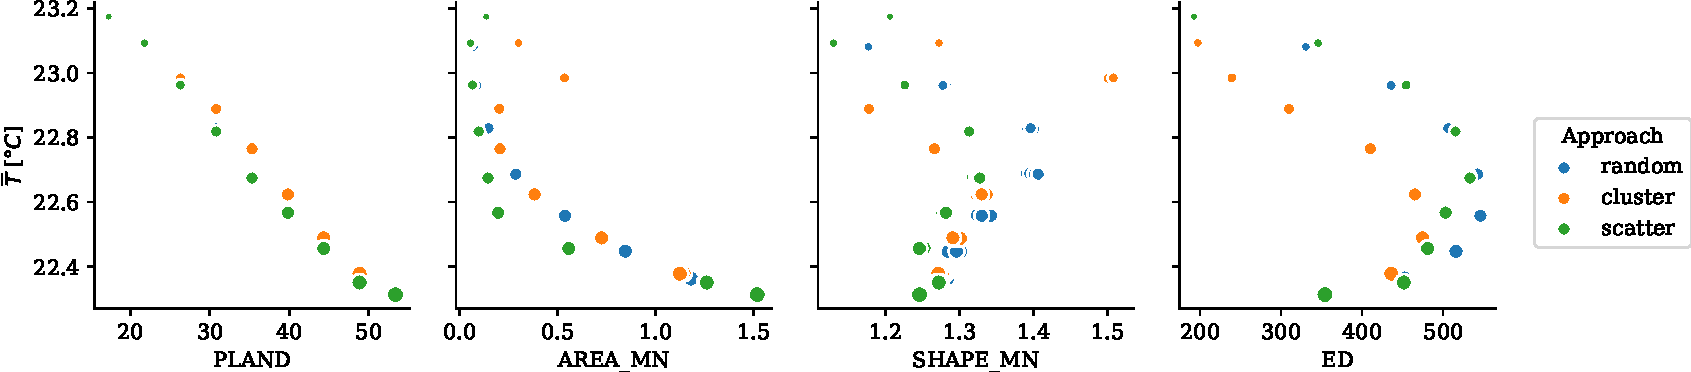
\includegraphics[width=1.4\textwidth]{figures/scenario-metrics.pdf}
    % \caption{\label{fig:scenario-metrics} Relationship between the percentage of pixels changed (out of the pixels where the tree canopy cover could be increased) and the resulting overall percentage of pixels with high tree canopy cover (left), mean patch size (MPS, in hectares) of pixels high tree canopy cover (center) and edge density (ED, in m / hectare) of pixels high tree canopy cover (right). The markers correspond to the scenarios that have actually been simulated, i.e., a ``cluster'' and a ``scatter'' scenario for each percentage of pixels changed, which starts at 0~\% and successively increases 10~\% until reaching a 100~\% of pixels changed (out of the pixels where the tree canopy cover could be increased).}
    \caption{\label{fig:scenario-metrics} Relationship between the percentage of landscape with high tree canopy cover (PLAND) and the mean patch size (MPS, in hectares, in the left sub-plot), the edge density (ED, in m / hectare, in the center sub-plot) and the mean shape index (MSI, adimensional, in the right sub-plot). The markers correspond to the scenarios that have actually been simulated, i.e., a ``cluster'' and a ``scatter'' scenario for each percentage of pixels changed, which starts at 0~\% and successively increases 10~\% until reaching a 100~\% of pixels changed (out of the pixels where the tree canopy cover could be increased). For each percentage of pixels changed, See \nameref{code-scenarios}.}
  \end{adjustwidth}
\end{figure}



\begin{figure}[ht]
  \begin{adjustwidth}{-.4\textwidth}{0cm}
    \centering
    % \includegraphics[width=1.4\textwidth]{figures/scenario-maps.pdf}
    \caption{\label{fig:scenario-maps} Comparison between the ``cluster'' and ``scatter'' scenarios for a proportion of changed pixels of 20~\%, i.e., a percentage of landscape with high tree canopy cover (PLAND) of . The blue points represent pixels that have high tree canopy cover in the ``cluster'' scenario but not in the ``scatter'', while orange points represent the converse. See \nameref{code-scenarios}.}
  \end{adjustwidth}
\end{figure}
  
% In the reference LULC raster map, the pixels with high tree canopy cover account for a 27~\% of the spatial extent of the study. After increasing the tree canopy cover in all the pixels where that is possible, such proportion raises to an overall 32.5~\%.
In the reference LULC raster map, the pixels with high tree canopy cover account for a 17.3~\% of the spatial extent of the study. After increasing the tree canopy cover in all the pixels where that is possible, such proportion raises to an overall 29.9~\%.
% Regarding the resulting percentage of pixels with high tree cover, there are no significant differences when 


\section*{Discussion}



\section*{Conclusion}


\section*{Supporting Information}

\subsection*{Table S1}
\label{table-station-locations}

% Location of the air temperature measurement stations, as comma-separated values (CSV).
% \url{https://github.com/martibosch/lausanne-heat-islands/blob/master/data/raw/tair-stations/station-locations.csv}
Air temperature measurement stations with their operator and their elevation in meters above sea level. The operators are: Agrometeo, Federal roads office (ASTRA), Federal office for the environment (BAFU), General directorate for the environment of the Canton of Vaud (DGE), and the Federal Institute of Forest, Snow and Landscape Research (WSL) \cite{rebetez2018meteorological}. The source comma-separated value (CSV) file used in the computational workflow is available at \url{https://github.com/martibosch/lausanne-heat-islands/blob/master/data/raw/tair-stations/station-locations.csv}.

\begin{table}[H]
  \begin{center}
    \begin{tabular}{ p{.3\textwidth} p{.15\textwidth} c }
      \toprule
      Station & Operator & Elevation [m.a.s.l] \\
      \midrule
      Bourg-en-Lavaux & Agrometeo & 519 \\
      Marcelin & Agrometeo & 436 \\
      Chandel M/13 & ASTRA & 680 \\  
      Morges & ASTRA & 380 \\
      Sorges & ASTRA & 500 \\
      Lausanne C\'esar-Roux & BAFU & 426 \\
      Bussigny & DGE & 429 \\
      Lausanne Plaines-du-Loup & DGE & 598 \\
      Morges & DGE & 376 \\
      Pully & MeteoSwiss & 426 \\
      Lausanne Freiland & WSL & 795 \\
      \bottomrule
    \end{tabular}
  \end{center}
  % \caption{\label{tab:stations} Air temperature measurement stations with their operator and their elevation in meters above sea level. The operators are: Agrometeo, Federal roads office (ASTRA), Federal office for the environment (BAFU), General directorate for the environment of the Canton of Vaud (DGE), and the Federal Institute of Forest, Snow and Landscape Research (WSL) \cite{rebetez2018meteorological}. The source comma-separated value (CSV) file used in the computational workflow is available at \url{https://github.com/martibosch/lausanne-heat-islands/blob/master/data/raw/tair-stations/station-locations.csv}.}
  % \textbf{Table S2.} Air temperature measurement stations with their operator and their elevation in meters above sea level. The operators are: Agrometeo, Federal roads office (ASTRA), Federal office for the environment (BAFU), General directorate for the environment of the Canton of Vaud (DGE), and the Federal Institute of Forest, Snow and Landscape Research (WSL) \cite{rebetez2018meteorological}. The source comma-separated value (CSV) file used in the computational workflow is available at \url{https://github.com/martibosch/lausanne-heat-islands/blob/master/data/raw/tair-stations/station-locations.csv}.
\end{table}


\subsection*{Table S2}
\label{table-biophysical}

% Biophysical table (before the reclassification), as comma-separated values (CSV).
% \url{https://github.com/martibosch/lausanne-heat-islands/blob/master/data/raw/biophysical-table.csv}
Biophysical table (before the reclassification). The crop and water coefficients are based on Allen et al. \cite{allen1998crop}, while rock, soil and urban coefficients are derived from the results of Grimmond and Oke \cite{grimmond1999evapotranspiration} in the city of Chicago. Given that the evapotranspiration of the vegetation and crops is subject to seasonal changes in temperate zones such as Switzerland \cite{allen1998crop}, the values that correspond to the mid-season estimation (June to August) in \cite{nistor2016mapping}.
The albedo values are based on the work of Steward et al. \cite{stewart2012local}.
The shade column, which represents the proportion of tree cover of each LULC class, is computed after the reclassification procedure described in \autoref{sec:refin-lulc-class}.
The source comma-separated value (CSV) file used in the computational workflow is available at \url{https://github.com/martibosch/lausanne-heat-islands/blob/master/data/raw/biophysical-table.csv}.

\begin{table}[H]
  \begin{adjustwidth}{-.02\textwidth}{0cm}  
    \begin{center}
      \begin{tabular}{ c p{.28\textwidth} p{.16\textwidth} c c c }
        \toprule
        LULC code & Description & Case & $K_c$ & Albedo & Green area \\
        \midrule
        0 & building & artificial & 0.4 & 0.1-0.25 & 0 \\ % 0.142
        1 & road, path & artificial & 0.35 & 0.15 & 0 \\ % 0.141
        2 & sidewalk & artificial & 0.35 & 0.15 & 0 \\
        3 & traffic island & artificial & 0.35 & 0.15 & 0 \\
        4 & rail & artificial & 0.35 & 0.15 & 0 \\
        5 & airfield & artificial & 0.4 & 0.2 & 0 \\
        6 & pond & water & 0.45 & 0.15 & 0 \\
        7 & other impervious & artificial & 0.36 & 0.15 & 0 \\
        8 & field, meadow, pasture & vegetation & 0.9 & 0.2 & 1 \\
        9 & vineyards & vegetation & 0.7 & 0.2 & 1 \\
        10 & other intensive farming & vegetation & 1.05 & 0.2 & 1 \\
        11 & garden & artificial & 0.32 & 0.2 & 1 \\
        12 & wetland & water & 0.45 & 0.1 & 1 \\
        13 & other green & vegetation & 0.45 & 0.2 & 1 \\
        14 & backwater & water & 0.65 & 0.05 & 1 \\
        15 & water course & water & 0.65 & 0.05 & 0\\
        16 & reed & water & 0.45 & 0.1 & 1\\
        17 & dense forest & vegetation & 1.5 & 0.15 & 1 \\
        18 & densely wooded pasture & vegetation & 1.15 & 0.15 & 1 \\
        19 & open wooded pasture & vegetation & 1.15 & 0.2 & 1 \\
        20 & other wooded & vegetation & 1.15 & 0.15 & 1\\
        21 & bare rocks & rock and soil & 0.2 & 0.25 & 0 \\
        22 & glacier & water & 0.52 & 0.1 & 0 \\
        23 & sand & rock and soil & 0.3 & 0.25 & 0 \\
        24 & gravel pit & artificial & 0.36 & 0.25 & 0 \\
        25 & other non-vegetated & artificial & 0.36 & 0.15 & 0 \\
        \bottomrule
      \end{tabular}
      % \caption{\label{tab:evapotranspiration-coefficients}
      % Evapotranspiration coefficients for each LULC class (see \nameref{table-biophysical}). Crop and water coefficients are based on Allen et al. \cite{allen1998crop}, while rock, soil and urban coefficients are derived from the results of Grimmond and Oke \cite{grimmond1999evapotranspiration} in the city of Chicago. Given that the evapotranspiration of the vegetation and crops is subject to seasonal changes in temperate zones such as Switzerland \cite{allen1998crop}, the values that correspond to the mid-season estimation (June to August) in \cite{nistor2016mapping}.
      % The albedo values are based on the work of Steward et al. \cite{stewart2012local}.
      % The source comma-separated value (CSV) file used in the computational workflow is available at \url{https://github.com/martibosch/lausanne-heat-islands/blob/master/data/raw/biophysical-table.csv}.
      % }
    \end{center}
    % \vspace{.5em}
    % \textbf{Table S3.} Biophysical table. The crop and water coefficients are based on Allen et al. \cite{allen1998crop}, while rock, soil and urban coefficients are derived from the results of Grimmond and Oke \cite{grimmond1999evapotranspiration} in the city of Chicago. Given that the evapotranspiration of the vegetation and crops is subject to seasonal changes in temperate zones such as Switzerland \cite{allen1998crop}, the values that correspond to the mid-season estimation (June to August) in \cite{nistor2016mapping}.
    % The albedo values are based on the work of Steward et al. \cite{stewart2012local}.
    % The source comma-separated value (CSV) file used in the computational workflow is available at \url{https://github.com/martibosch/lausanne-heat-islands/blob/master/data/raw/biophysical-table.csv}.
  \end{adjustwidth}
\end{table}


\subsection*{Code S4}
\label{code-reclassification}
Reclassification details, as Jupyter Notebook (IPYNB).
\url{https://github.com/martibosch/lausanne-heat-islands/blob/master/notebooks/reclassification.ipynb}

\subsection*{Code S5}
\label{code-scenarios}
Scenario generation details, as Jupyter Notebook (IPYNB).
\url{https://github.com/martibosch/lausanne-heat-islands/blob/master/notebooks/scenarios.ipynb}

\section*{Acknowledgments}
This research has been supported by the \'Ecole Polytechnique F\'ed\'erale de Lausanne (EPFL).

\nolinenumbers

% This is where your bibliography is generated. Make sure that your .bib file is actually called library.bib
\bibliography{references}

%This defines the bibliographies style. Search online for a list of available styles.
\bibliographystyle{unsrt}

\end{document}
